\documentclass[11pt]{article}
\usepackage[a4paper,margin=25mm]{geometry}
\usepackage{amsmath,amssymb,amsthm,booktabs,graphicx,xcolor}
\usepackage[numbers,sort&compress]{natbib}
\usepackage{xr-hyper}
\usepackage[hidelinks]{hyperref}
\externaldocument[][nocite]{sod_rom_v5}
% shared macros for the SOD tutorial and papers
% Typesetting follows ISO 80000-2: italic scalars (capital Greek via \var...),
% bold italic vectors and matrices (\bm), upright d, e, i, operators and labels.
\usepackage{bm,upgreek}
\newcommand{\bx}{\bm{x}}  \newcommand{\bz}{\bm{z}}  \newcommand{\bX}{\bm{X}}
\newcommand{\bV}{\bm{V}}  \newcommand{\bW}{\bm{W}}  \newcommand{\bU}{\bm{U}}
\newcommand{\bM}{\bm{M}}  \newcommand{\bK}{\bm{K}}  \newcommand{\bC}{\bm{C}}
\newcommand{\bA}{\bm{A}}  \newcommand{\bB}{\bm{B}}  \newcommand{\bS}{\bm{S}}
\newcommand{\bI}{\bm{I}}  \newcommand{\bff}{\bm{f}}
\newcommand{\bSig}{\bm{\varSigma}}  \newcommand{\bpsi}{\bm{\psi}}  \newcommand{\bPsi}{\bm{\varPsi}}
\newcommand{\bphi}{\bm{\phi}}  \newcommand{\bPhi}{\bm{\varPhi}}
\newcommand{\avg}[1]{\left\langle #1 \right\rangle}
\newcommand{\bnd}[1]{\left[ #1 \right]_T}
\newcommand{\sym}{\operatorname{sym}}  \newcommand{\skw}{\operatorname{skew}}
\newcommand{\TODO}[2]{\textcolor{red}{\textbf{[#1]} #2}}

\graphicspath{{../figures/}}
\setlength{\emergencystretch}{3em}
\renewcommand{\thesection}{S\arabic{section}}
\renewcommand{\thefigure}{S\arabic{figure}}
\renewcommand{\thetable}{S\arabic{table}}
\renewcommand{\theequation}{S\arabic{equation}}
\title{Supplementary material for\\ ``What a free decay teaches a smooth orthogonal decomposition basis''}
\author{David Chelidze\\ Nonlinear Dynamics Laboratory, University of Rhode Island}
\date{}
\begin{document}
\maketitle
\noindent Section, figure, table and equation numbers without the prefix S refer to the main text. Every number below is produced by the scripts named in Appendix~B of the main text.

\noindent Sections~\ref{sec:acc}--\ref{sec:s-noise} hold the forced-record study that Section~\ref{sec:contrast} summarizes. Section~\ref{sec:complex} holds the complex-mode and state-space study, Sections~\ref{sec:s-s4} and \ref{sec:s-s5} the details of the two nonlinear cantilevers, and Section~\ref{sec:cost} the integration cost.

\section{Forced training records: errors against order}\label{sec:acc}
Does an SOD basis improve on the LNMs and on MTA, and at which orders?
Figure~\ref{fig:error} shows the median error and interquartile range against state dimension.
Away from the data rank the interquartile range was at most 0.76 of the median. Ratios between bases below are therefore meaningful. Near the rank, and for state SOD at $c_{\mathrm d}=1$, it reached 5.3.
The data rank of random records varied between realizations, for example 8--9 on S2 with light damping. A median is reported only at orders that all 20 realizations supply.

\paragraph{Low order: SOD is the LNM basis; POD from forced data is not.} At $r=1$ and 2, SOD from random or free-decay data matched the LNM ROM within 15\,\% on S1 and S2.
POD from forced data did not on S2; on S1 it matched as well. Take S2 with light damping and one mode from random data. POD erred by $2.2\times10^{-1}$ on the training load, against $1.1\times10^{-1}$ for the LNM. On the free-decay test it erred by $2.0\times10^{-1}$ against $1.1\times10^{-2}$.
Swept-sine SOD failed at $r=2$ on S2 with light damping: $1.5\times10^{-1}$ against $1.9\times10^{-2}$ (Section~\ref{sec:mix}).

\paragraph{Intermediate order: the random-trained basis falls behind.} At $r=3$--4, SOD from random data was worse than the LNMs on S2. It was 4.8 times worse at $r=3$ on the training load, and 18 times worse at $r=4$ at mid-span.
Free-decay SOD was not. On S2 with light damping, BL and SR bases matched the LNMs within 4\,\% through $r=5$.

\paragraph{High order, training load: data beat the LNMs, and match or beat MTA.} At $r=8$, SOD from random data erred by:
\begin{itemize}
\item S1: $4.3\times10^{-5}$ (light) and $1.7\times10^{-6}$ (heavy), against LNM $2.3\times10^{-4}$ and $6.3\times10^{-4}$, and MTA $4.6\times10^{-5}$ and $3.7\times10^{-5}$;
\item S2: $1.6\times10^{-6}$ (light) and $1.9\times10^{-7}$ (heavy), against LNM $4.2\times10^{-5}$ and $1.2\times10^{-4}$, and MTA $1.1\times10^{-5}$ and $1.8\times10^{-5}$.
\end{itemize}
POD gave nearly the same values. On S1 and S2 with heavy damping, $r=8$ is the data rank. There SOD and POD span one subspace and give identical ROMs.
The gain over the LNMs comes from the quasi-static response of truncated modes, which a forced record contains. MTA adds that response from the model as the static deflection under each load, one vector per load location.

\begin{figure}[tbp]
\centering
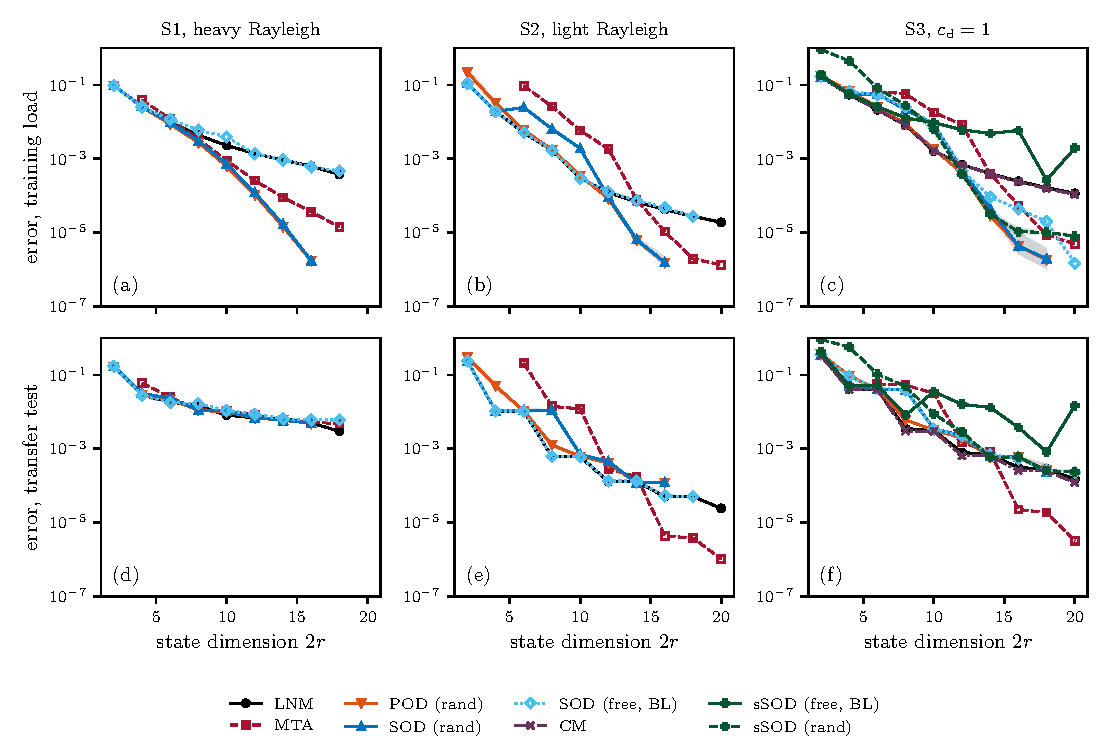
\includegraphics[width=\textwidth]{fig_c_error.pdf}
\caption{ROM displacement error against state dimension $2r$, median and interquartile range over 20 realizations. Columns: S1 with heavy Rayleigh damping; S2 with light Rayleigh damping; S3 with $c_{\mathrm d}=1$. Top: new random load at the training location. Bottom: transfer test (free decay from a floor-4 point load for S1; random mid-span load for S2 and S3). Training signal in brackets; free, BL: order-matched band-limited decay; sSOD: state-space SOD; CM: complex-mode truncation.}
\label{fig:error}
\end{figure}
So the same random-trained basis is worse than the LNMs at intermediate order and better at high order, and the gain belongs to the training load. Sections~\ref{sec:adds} and \ref{sec:displace} explain both.

\section{Forced training records: what the record adds}\label{sec:adds}
Is the high-order gain of a random-trained SOD basis the static correction, and does it serve only the loads the record saw?
We answer first by the geometry of the basis and then by moving the load.

\paragraph{Containment of the static vectors.} Figure~\ref{fig:static}a gives the containment residual \eqref{eq:contain} of the two static load vectors of S2, $\bK^{-1}\bm{b}_{\mathrm{tip}}$ and $\bK^{-1}\bm{b}_{\mathrm{mid}}$, with light damping and the 20 random tip records of Section~\ref{sec:acc}.
\begin{itemize}
\item At $r=8$ the SOD subspace holds the tip vector to $\rho=1.8\times10^{-7}$ (median), against $3.3\times10^{-5}$ for the LNMs, about 190 times closer. At $r=7$ the figures are $1.6\times10^{-6}$ and $5.2\times10^{-5}$.
\item It holds the mid-span vector no better than the LNMs: $7.9\times10^{-5}$ against $3.7\times10^{-5}$ at $r=8$. The record never saw that load.
\item The SOD basis of the order-matched band-limited decay contains no static correction. Its residuals equal those of the LNMs within 12\,\% ($3.6\times10^{-5}$ for the tip vector at $r=8$), as its LNM-level errors in Figure~\ref{fig:error} require.
\end{itemize}
POD of the same records contained the tip vector equally well ($1.7\times10^{-7}$ at $r=8$). At the data rank the two span one subspace.

\paragraph{Principal angles.} At $r=8$, seven of the eight principal angles between the SOD subspace and MTA with the tip vector only were below $0.03^\circ$ (medians); the eighth was $13^\circ$ (at most $15^\circ$). Against the eight LNMs, six angles were below $0.01^\circ$, then $2^\circ$ and $50^\circ$. Against MTA with both static vectors, the largest angle was $69^\circ$, because the mid-span vector is missing.
The random record thus supplies the LNMs it excites and, in place of LNM~8, the static correction of the load it saw.

\begin{figure}[tbp]
\centering
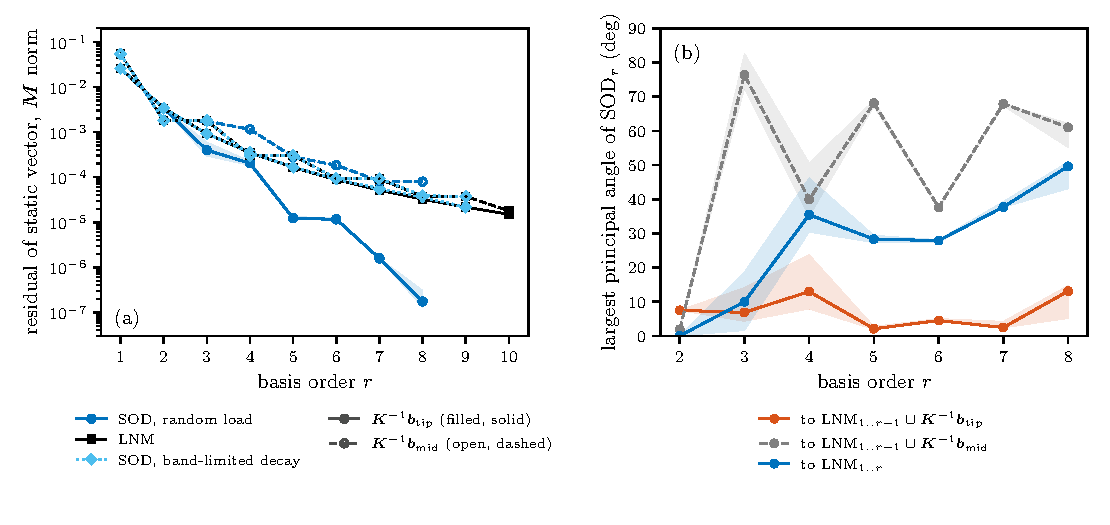
\includegraphics[width=\textwidth]{fig_c_static.pdf}
\caption{What a random tip record adds to the SOD basis; S2, light Rayleigh damping, 20 realizations. (a) Containment residual \eqref{eq:contain} of the static load vectors $\bK^{-1}\bm{b}_{\mathrm{tip}}$ (filled, solid) and $\bK^{-1}\bm{b}_{\mathrm{mid}}$ (open, dashed) against the basis order $r$: SOD of the random tip records (median and interquartile range), LNMs, and SOD of the order-matched band-limited decay. (b) Largest principal angle ($\bM$ metric) between the first $r$ SOD directions and the first $r$ LNMs, and between them and the first $r-1$ LNMs augmented by one static vector; median and range. Scripts: \texttt{g1\_static\_containment.py}, \texttt{g3\_third\_direction.py}, \texttt{mkfig\_c\_static.py}.}
\label{fig:static}
\end{figure}

\paragraph{Transfer: the gain stays at the load locations each basis was given.} For a random load at mid-span, the bases trained at the tip lost their advantage. MTA as defined above contains the static vector of the mid-span load. We therefore also built MTA with the tip vector only. We also trained data bases on independent random loads at both locations. At $r=8$ on the mid-span test:
\begin{itemize}
\item tip only: SOD erred by $1.2\times10^{-4}$ (S2, light) and $3.1\times10^{-4}$ (S2, heavy). MTA with the tip vector erred by $1.1\times10^{-4}$ and $2.9\times10^{-4}$, and the LNMs by $4.8\times10^{-5}$ and $1.4\times10^{-4}$;
\item both locations: SOD erred by $6.0\times10^{-6}$ and $9.0\times10^{-6}$; MTA by $4.2\times10^{-6}$ and $7.9\times10^{-6}$.
\end{itemize}
On S3 the pattern held. SOD and MTA from one location erred by $2.7$--$6.0\times10^{-4}$. From both locations, MTA erred by $1.0$--$2.3\times10^{-5}$ and SOD by $1.9$--$7.8\times10^{-5}$.
So on S2 and S3, SOD and MTA gained at the same load locations: those each basis was given. SOD needs response records at those locations.
On S2 at $r=7$, SOD and LNM were within 10\,\% of each other. The LNM curve for the mid-span load is a staircase, flat at $r=3$, 5 and 7. Mid-span lies within 2\,\% of a node of modes 3, 5 and 7.
On S1 the transfer test, a free decay from a point load at floor 4, was nearly basis-independent. All bases stayed within a factor of 2.1 of one another for $r=3$--9. None was consistently best.
MTA is not uniformly better. On the S2 free-decay test it was 44 times worse than the LNMs at $r=3$. At $r=8$ it was about twice as poor. On S1 it did not beat the LNMs on the floor-4 decay.
The data-driven gain is the persistence problem of \citet{Ilbeigi2017}, seen in a linear system: on S2 and S3 the data bases gained only at the load locations of their records.

\paragraph{Noisy training records.} The gain above used model kinematics. With white noise of 60 or 40\,dB on the training displacements the S2 error stopped falling at $r=6$--7, and the high-order gain was lost (Section~\ref{sec:s-noise}).

\section{Forced training records: why low orders fail}\label{sec:displace}
Why is the random-trained basis worse than the LNMs at $r=3$--5, when it holds the useful direction?
Figure~\ref{fig:static}b and the LNM content of each SOD subspace answer it.

\paragraph{One direction, ranked too early.} The SOD subspace of order $r$ held only $r-1$ LNMs for $r=3$--7 (median $\bM$-residual of each LNM below 0.1). At $r=3$ it held modes 1 and 2; LNM~3 had residual 0.17. At $r=5$ it held modes 1--4, and at $r=6$ modes 1--5, all the modes inside the load band.
The extra direction is the tip static correction. From $r=3$ on, the SOD subspace lay within $2$--$13^\circ$ (medians) of the first $r-1$ LNMs augmented by $\bK^{-1}\bm{b}_{\mathrm{tip}}$. It lay $10$--$50^\circ$ from the first $r$ LNMs, and $38$--$76^\circ$ from the first $r-1$ LNMs augmented by the mid-span vector (Figure~\ref{fig:static}b).
The direction enters at $r=3$ because it is smoother than the upper in-band modes: the third SOD frequency of a random record was 47.7, between modes 2 and 3 (Section~\ref{sec:mix}).
The errors follow the count of in-band modes. Against the LNM ROM the SOD ROM was 4.8 times worse at $r=3$ and 6.5 times worse at $r=5$, while it lacked one in-band mode. At $r=6$, with all five in-band modes present, it was 1.4 times better. At $r=7$ and 8 it was 11 and 27 times better.
The direction that carries the gain at high order is the one that causes the loss at low order.

\subsection{Mixing by training signal}\label{sec:mix}
The same ranking explains how the training signal shapes the basis.
Figure~\ref{fig:mac} compares configuration SOD modes with LNMs by the mass-weighted modal assurance criterion (MAC; \citealp{Allemang2003}; one realization).
\begin{itemize}
\item \emph{Free decay, proportional damping.} On S2, SOD modes 1--8 matched LNMs 1--8 with MAC $\ge0.93$. Frequencies of modes 1--6 were within 0.03--1.6\,\%. The modal coordinates were nearly uncorrelated (largest correlation 0.07).
\item \emph{Random and swept sine.} Extra smooth directions appeared between genuine modes. On S2 with random data, SOD returned frequencies 3.5, 22.0, 47.7, 62.2, 121, 200. The third is a mixture of LNMs 1--3 (MAC 0.19, 0.28, 0.51): the quasi-static tip direction of Section~\ref{sec:displace}. The sweep inserted a direction at 17.1, below mode 2.
\item \emph{Free decay with the dashpot.} Non-proportional damping correlates the modal coordinates (0.71). Configuration SOD modes 2--4 mixed (MAC 0.82, 0.86, 0.58), as the exactness criterion predicts.
\end{itemize}
Every direction ranked among the modes shifts the genuine modes down one rank. A truncated basis then omits a mode it needs, which explains the intermediate-order errors.
State-space SOD on S3 behaves in the same way, plane by plane (Section~\ref{sec:s-smix}).

\begin{figure}[tbp]
\centering
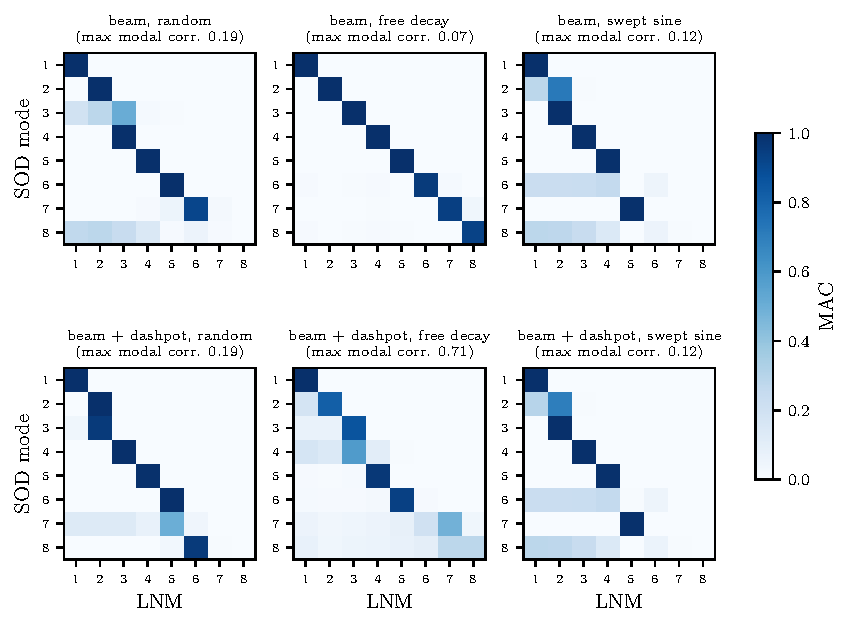
\includegraphics[width=0.92\textwidth]{fig_c_mac.pdf}
\caption{MAC between configuration SOD modes 1--8 (rows, smoothest first) and LNMs 1--8 (columns); the training data excite no higher modes. Top: S2, light damping. Bottom: S3, $c_{\mathrm d}=0.2$. Columns: training signal.}
\label{fig:mac}
\end{figure}

A free decay under proportional damping avoids the displacement, because it contains no quasi-static response. A forced record contains it, and ranking by smoothness misplaces it.

\subsection{Sensitivity to the retained rank}\label{sec:rank}
Smaller rank tolerances admit a second kind of smooth non-modal direction: weakly excited ones. They depend on how much of the near-null data space is kept.
For S2 under a random tip load, POD eigenvalues fall from 1 to $1.7\times10^{-9}$ over eight directions. They then drop to $9\times10^{-12}$ and below.
\begin{itemize}
\item tolerance $10^{-6}$ (rank 6): modes 1--4 clean, mode 5 mixed;
\item tolerance $10^{-10}$ (rank 8): a spurious direction at 46.5 between modes 2 and 3;
\item tolerance $10^{-12}$--$10^{-14}$ (rank 10--11): spurious directions at 1.0--1.7, smoother than mode 1.
\end{itemize}
The spurious directions carried energy fractions of $6\times10^{-5}$--$3\times10^{-4}$, comparable to the fourth and fifth LNM components. An energy threshold therefore cannot separate them.
Weakly excited directions can look smooth. Their mean-square frequency is set by how little they move, not by a mode.
We observed them in clean, band-limited records. Section~\ref{sec:noise} shows how to recognise the genuine modes.

\section{Forced training records: recognising modes}\label{sec:noise}
How can the quasi-static direction be kept without letting it displace a mode?
For model reduction the kinematics come from the model: velocities and state derivatives are exact, and no measurement noise enters.
Modes are therefore recognised, paired and ordered by their own frequency or circularity, never by their SOD value. Smoothness says how slowly a projection moves. It does not say which mode the projection belongs to, as Sections~\ref{sec:displace} and \ref{sec:rank} show.

\subsection{Recognising modes}\label{sec:recog}
\paragraph{Configuration SOD: spectral consistency.} A coordinate that is a single real mode has its mean-square frequency at its spectral peak. A mixture of modes does not. We read each coordinate's spectrum from its periodogram of the type-II discrete cosine transform (DCT-II), smoothed over $\pm2\,\%$ in frequency. A raw periodogram of a randomly forced coordinate has single-bin spikes. Its arg-max is then not the resonance, and its bin-level width misses the damping width $2\zeta\omega$. Coordinate $i$ is kept if its peak lies within $\max(5\,\%,\,w_i)$ of its SOD frequency $\sqrt{\mu_i}$. Here $w_i$ is the relative half-power width of that peak, capped at 15\,\%. The width makes the test damping-aware. The cap matters. A drifting or broadband coordinate peaks near zero frequency, with a width above 1, and would otherwise pass. The test assumes one frequency per coordinate. A nonlinear decay sweeps that frequency, and the test can then reject a genuine NNM (Section~\ref{sec:nlbb}). Circularity needs no fixed frequency. Two kept coordinates that share one peak cannot both be that mode. The one carrying more response energy, $\|\bphi_i\|^2\avg{q_i^2}$, is kept. Recognised modes are ordered by peak frequency.
Applied with a fixed 5\,\% tolerance to the ten smoothest coordinates of clean S2 records, the test rejected 108 of 134 spurious directions and no genuine mode (10 realizations, tolerances $10^{-10}$--$10^{-14}$). Two other rules did worse. A two-halves rule keeps a coordinate if SOD of each half of the record returns a smooth mode with MAC above 0.9 and frequency within 5\,\% of it; it rejected 102 spurious directions and also 10 of 147 genuine modes. A lag-diagonality rule keeps a coordinate if its lagged correlation with every other coordinate stays below 0.3 at lags of 1/16 to 1/2 of its own period; it rejected 40 and 13 (\texttt{c19\_selection\_rules.py}).

\paragraph{State SOD: circularity.} Consider the two coordinates of a modal plane. Up to a real change of basis, they are the real and imaginary parts of one complex modal coordinate. SOD returns them uncorrelated and with unit variance, so in their own plane the cloud is round. Read as $z=q_a+\mathrm i\,q_b$, the pair rotates one way and the spectrum of $z$ is one-sided. Two unrelated coordinates, or coordinates of two different planes, give a nearly symmetric spectrum.
Pairs are therefore formed by matching, not by rank. Candidate pairs are paired greedily by one-sidedness and kept above 0.85; only one plane is kept per frequency. A loose frequency gate, four times the spectral tolerance, only limits the search. The plane frequency is the peak of the one-sided spectrum of $z$, and planes are ordered by it.
Pairing by rank fails. Pairing adjacent coordinates in SOD order lost the slowest plane of random-load records, because a quasi-static coordinate sat between its two members. Requiring the two members' raw spectral peaks to agree lost it in 4 of 10 records, because those peaks scattered by up to 21\,\% under random forcing. With smoothed spectra and the loose gate, the mode-1 plane was recognised in all 8 test records. Modal planes gave a one-sidedness of 0.89--0.99, other pairs 0.51--0.75. A strong plane can be contaminated by another mode at its own frequency, which lowers its one-sidedness. A pair scoring 0.75--0.85 is therefore also kept under two conditions. Its one-sidedness within $\pm30\,\%$ of its peak must be at least 0.95. It must also carry at least 1\,\% of the response energy. The banded test alone is unsafe. On noisy linear records it admitted up to 15 times more non-modal pairs. Two narrowband noise coordinates in quadrature also look circular. With the energy gate, the model-reduction results did not change. From one random-load record on S3 ($c_{\mathrm d}=0.2$) the recognised planes were at 3.7, 22.1, 62.5, 121.2 and 201.4. From the band-limited decay they were at 3.5, 22.0, 61.7, 120.9 and 199.6. The damped frequencies are 3.5, 22.0, 61.7, 120.9 and 199.7.

\subsection{Selection for model reduction}\label{sec:romsel}
We compared two bases from the same SOD, with model kinematics (10 realizations):
\begin{itemize}
\item R0: the plain basis, in SOD order;
\item RHB: the recognised modes or planes inside the load band, $\omega\le\omega_{\mathrm c}$, first, ordered by frequency; then the remaining coordinates in SOD order.
\end{itemize}
Section~\ref{sec:s-recog} compares four other orders.
Modes above the load band respond quasi-statically to it. The smooth direction that carries that response serves a ROM better than the mode itself. This is why RHB stops at $\omega_{\mathrm c}$.
\paragraph{S2, random tip load.} RHB removed the low-order damage of spurious directions. In no record was it more than 11\,\% worse than R0 at any order.
\begin{itemize}
\item Tolerance $10^{-12}$: the median two-mode error fell from $1.1\times10^{-1}$ to $2.0\times10^{-2}$ on the training load. At mid-span it fell from $2.2\times10^{-1}$ to $1.0\times10^{-2}$. The four-mode errors fell from $6.1\times10^{-3}$ to $1.8\times10^{-3}$ and from $1.0\times10^{-2}$ to $6.5\times10^{-4}$.
\item Tolerance $10^{-10}$: the four-mode mid-span error fell from $1.1\times10^{-2}$ to $7.6\times10^{-4}$.
\item At $r=6$ RHB equalled R0 at tolerance $10^{-10}$ and improved it at $10^{-12}$ ($1.7\times10^{-4}$ to $1.0\times10^{-4}$ on the training load). At $r=8$ all bases erred by $1.4\times10^{-6}$ on the training load.
\end{itemize}
\paragraph{S3, $c_{\mathrm d}=0.2$, state SOD.} From random-load records RHB improved state dimension 4 in every record (median training-load error $2.9\times10^{-1}\to1.0\times10^{-1}$, mid-span $3.7\times10^{-1}\to9.2\times10^{-2}$). At state dimension 8 it was slightly worse (median ratio 1.1--1.2, at most 2.5 in one record). From 12 on it equalled R0. Planes from forced records are tilted by their quasi-static response (Section~\ref{sec:ic}). From the band-limited decay the recognised order matched the SOD order, and all bases were identical.
For model reduction we therefore recommend RHB. Recognised in-band modes come first, by frequency; the rest follow in SOD order.
Recognition thus keeps the static-correction direction in the basis but places it behind the in-band modes it displaced.

\subsection{Other orders}\label{sec:s-recog}
\paragraph{Two other recognition orders.}
\begin{itemize}
\item RID: the recognised modes or planes only, up to $1.2\,\omega_{\mathrm c}$, ordered by frequency;
\item RH: the recognised modes first, by frequency, then the remaining coordinates in SOD order;
\end{itemize}
RH also puts the recognised mode 6 (frequency about 295) first. It was 1.3--10 times worse than R0 on the training load at $r=6$ and tolerance $10^{-10}$, though better at mid-span. RID alone stops at the six modes below $1.2\,\omega_{\mathrm c}$.
\paragraph{Can a frequency place the other coordinates?} Two further orders placed every coordinate by a frequency.
\begin{itemize}
\item RF: recognised modes at their peak frequency, all other coordinates at their SOD frequency $\sqrt{\mu}$.
\item RQ: every coordinate at the Rayleigh-quotient frequency of its displacement shape, $\sqrt{\bphi^{\mathsf T}\bK\bphi/\bphi^{\mathsf T}\bM\bphi}$, from the model. For state SOD both members of a plane take the geometric mean of their two values.
\end{itemize}
RF gave the same ROMs as R0 in every record (S2 at both tolerances, S3 at $10^{-10}$). The SOD frequency of a quasi-static direction follows the load spectrum, not the structure. Here it never moved past a mode.
RQ was no better than R0 at $r=6$ and 8 on S2. The median ratio was 1.0--4.0 at tolerance $10^{-10}$ and 1.0--57 at $10^{-12}$. On S3 it was worse from state dimension 12. The median ratio was 1.3--220 on random records; the ratio was 2.3--5.5 on the single band-limited decay.
At tolerance $10^{-12}$ it improved $r=2$ (median ratio 0.5--0.6), but RHB did as well or better. A quasi-static direction is stiff, so RQ moves it to the end of the basis. A ROM of low order then cannot use it.
The value of such a direction lies in its share of the forced response. The SOD order already measures that share.

\section{Load responses at the SOD frequencies: forced records}\label{sec:s-forced}
For the random tip-load training records of Section~\ref{sec:acc}, identity \eqref{eq:identity} of the main text holds with the load as the force. Table~\ref{tab:s-forced} compares the SOD ROM with the ROM on the model-built basis $\operatorname{span}\{\bm{d}(\sqrt{\mu_1}),\dots,\bm{d}(\sqrt{\mu_r})\}$, $\bm{d}(\omega)=(\bK-\omega^2\bM)^{-1}\bm{b}$, with the SOD frequencies taken from the same record (\texttt{i2\_interp\_basis.py}; 20 realizations, new random load at the training input). With light damping and with the tip dashpot the two agree within factors of 0.82--1.68. With heavy Rayleigh damping the model-built basis falls behind as the order grows, by 4.5 (S1) and 40 (S2) at $r=8$. The real parts of the damped responses $(\bK-\omega^2\bM+\mathrm i\omega\bC)^{-1}\bm{b}$ brought the S2 factor at $r=8$ to 2.0, but were 2.7--5.5 times worse than SOD at $r=1$ and 2, and did not help on S1 (5.1 at $r=8$; \texttt{i3\_damped\_basis.py}). What SOD holds beyond the undamped load responses under heavy proportional damping is not identified here.
The median angles between the smooth modes and $\bm{d}(\sqrt{\mu_i})$ were $0.001^\circ$, $0.017^\circ$, $5.0^\circ$, $0.54^\circ$ and $1.4^\circ$ for directions 1--5 of S2 with light damping; the third is the non-modal direction near 50 (\texttt{i1\_forced\_identity.py}).

\begin{table}[tbp]
\centering\small
\caption{Median over 20 realizations of the ROM error on the model-built basis of load responses at the SOD frequencies, divided by the SOD ROM error; random load at the training input. Smallest and largest value over $r=1$--8, and the value at $r=8$. Script: \texttt{i2\_interp\_basis.py}.}
\label{tab:s-forced}
\begin{tabular}{lccc}
\toprule
case & smallest & largest & $r=8$\\ \midrule
S1, light Rayleigh & 0.96 & 1.00 & 0.99\\
S2, light Rayleigh & 0.82 & 1.21 & 1.13\\
S3, $c_{\mathrm d}=0.2$ & 1.00 & 1.52 & 1.19\\
S3, $c_{\mathrm d}=1$ & 0.97 & 1.68 & 1.12\\
S1, heavy Rayleigh & 0.91 & 4.46 & 4.46\\
S2, heavy Rayleigh & 0.62 & 40.05 & 40.05\\
\bottomrule
\end{tabular}
\end{table}

\section{Noisy training records}\label{sec:s-noise}
The high-order gain of Section~\ref{sec:adds} used model kinematics. We repeated S2 with measured training records. All 60 displacements carried white noise at 60 or 40\,dB and were smoothed by Whittaker smoothing (WH; penalty on the third difference, 100\,Hz corner, one setting for all channels) \citep{Eilers2003}. Velocities came from the smoothed record (5 realizations).
\begin{itemize}
\item Noise removed the data rank, so the bases reached every order. Their error, however, stopped falling at $r=6$--7.
\item At $r=8$ on the training load, SOD erred by $1.4\times10^{-4}$ (light) and $2.5\times10^{-5}$ (heavy) at 60\,dB. At 40\,dB it erred by $1.4\times10^{-2}$ and $1.5\times10^{-3}$. With model kinematics it erred by $1.5\times10^{-6}$ and $2.0\times10^{-7}$.
\item At 60\,dB SOD was 3 times worse than the LNMs (light) or 5 times better (heavy). At 40\,dB it was 11--300 times worse. POD behaved the same.
\end{itemize}
The floor rose 100-fold for a 10-fold rise in noise amplitude. The high-order gain therefore needs clean training records. For model reduction they should come from the model.

\section{Complex modes and state-space SOD ROMs}\label{sec:complex}
On S3 the modes are complex, and configuration SOD from a free decay mixed modes 2--4 (MAC 0.82, 0.86 and 0.58; Section~\ref{sec:mix}). Complex modes themselves bought little on the forced tests: a configuration ROM on the undamped LNMs, with the full damping matrix projected, erred within 25\,\% of complex-mode truncation at every order (ratio 0.96--1.25). On the free test decay complex-mode truncation was 2.5--7 times better at state dimension 8. Configuration SOD fails on S3 because its modes mix, not because the true modes are complex.
State-space SOD of the order-matched band-limited decay mixed them much less. On the forced tests at state dimension 8 it came within a factor of 2.7 of complex-mode truncation, and it cut the mid-span error of configuration SOD by 5--13 times. Above state dimension 8 its error stalled near $10^{-3}$ on the random test: weakly excited planes are poorly determined by a decay. No energy-Galerkin state ROM was unstable.
The planes follow the record, as the configuration modes did. A decay tilts them toward the modes it excites above the retained band; where the leakage exceeded 0.05, the ROM converted it into a relative eigenvalue error of 0.2--0.8 times its square. Of the decays tested, those with little energy above the retained band, relative to the energy inside it, gave the most accurate state ROMs: static release, and band-limited decays matched to the ROM order. A forced record tilts the planes by its quasi-static response; state SOD from random records erred by $6.1\times10^{-1}$ at state dimension 2 ($c_{\mathrm d}=0.2$). Sections~\ref{sec:s-pg}--\ref{sec:ic} give the Petrov--Galerkin result, the dependence on the training signal, the errors per case, the trajectories and the training-decay study.

\subsection{Petrov--Galerkin state ROM}\label{sec:s-pg}
The Petrov--Galerkin state ROM of Section~\ref{sec:ssod} failed. Data covectors are undetermined outside the span of the data, and their input coupling $\|\bm{\psi}_i^{\mathsf T}\bm{B}_{\mathrm s}\|$ reached $2\times10^3$--$3\times10^5$. On S3 with tip-dashpot coefficient $c_{\mathrm d}=0.2$ and a free-decay basis, its error under a random load was 70 at every order.

\subsection{State-space SOD and the training signal}\label{sec:s-smix}
State-space SOD on S3 depends on the training signal as configuration SOD does (Section~\ref{sec:mix}), plane by plane. From the free decay at $c_{\mathrm d}=0.2$, the pairs 1--2, 3--4, 5--6 and 7--8 matched modal planes 1--4. Their geometric-mean frequencies were within 0.2--2\,\% of $|s_i|$, and the planes within $0.3$--$14^\circ$ in the energy metric. The inter-plane correlation of that decay was 0.14.
At $c_{\mathrm d}=1$ the correlation rose to 0.31, and plane 2 was off by $48^\circ$.
From random or swept-sine records, the smoothest state direction was not modal, and pairs mixed planes, as in configuration space.

\subsection{Errors per case and trajectories}\label{sec:s-complex}
At state dimension 8, with BL training (SR in brackets; Section~\ref{sec:ic} compares other decays):
\begin{itemize}
\item $c_{\mathrm d}=0.2$: state SOD erred by $4.6\times10^{-3}$ ($4.5\times10^{-3}$), $2.0\times10^{-3}$ ($2.1\times10^{-3}$) and $9.8\times10^{-4}$ ($2.2\times10^{-4}$) on the random, mid-span and SR-decay tests. Configuration SOD erred by $1.7\times10^{-2}$, $2.7\times10^{-2}$ and $6.5\times10^{-4}$, and complex-mode truncation by $4.3\times10^{-3}$, $1.5\times10^{-3}$ and $4.3\times10^{-5}$;
\item $c_{\mathrm d}=1$: state SOD $1.3\times10^{-2}$ ($9.0\times10^{-3}$), $8.0\times10^{-3}$ ($6.8\times10^{-3}$), $3.9\times10^{-3}$ ($5.9\times10^{-4}$); configuration SOD $2.5\times10^{-2}$, $3.9\times10^{-2}$, $7.7\times10^{-4}$; complex-mode truncation $8.2\times10^{-3}$, $3.0\times10^{-3}$, $5.6\times10^{-5}$.
\end{itemize}
Consider forced tests at state dimension 8. State SOD from the BL decay came within a factor of 2.7 of complex modes. At 10--16 the factor grew to 1.9--25. It was also within that factor of the LNM ROM (1.1--2.3). It cut the mid-span error of configuration SOD by 5--13 times (random tip test: 2--4). On the SR-decay test it stayed 20--70 times above the complex modes (SR training: 5--10 times). The planes are estimated from a short, correlated decay, and part of this gap is the initial-state projection (Section~\ref{sec:ic}).
Above state dimension 8 the BL state SOD error stalled near $10^{-3}$ on the random test. The SR basis kept improving, to $6.9\times10^{-5}$ at state dimension 16 for $c_{\mathrm d}=0.2$. Its error stopped falling above 14--16. On the mid-span test it rose already from 10 to 12, and at $c_{\mathrm d}=1$ it became erratic. Weakly excited planes are poorly determined by a decay.
State SOD from forced records was poor at low order: $6.1\times10^{-1}$ at state dimension 2 for $c_{\mathrm d}=0.2$. Its smoothest directions are forced, not modal (Section~\ref{sec:mix}).

\paragraph{Trajectories.} Figure~\ref{fig:traj} compares tip responses at state dimension 8 for one realization (seed 2026).
On S2 under the mid-span load, the LNM ROM overlays the full model. So does the SOD ROM from the equal-energy decay. Their errors were $5.7\times10^{-4}$ and $5.9\times10^{-4}$. Random-trained SOD and MTA erred by $1.0\times10^{-2}$ and $1.3\times10^{-2}$; at $r=4$ MTA keeps only two LNMs.
On S3 with $c_{\mathrm d}=1$, complex-mode truncation erred by $2.9\times10^{-3}$. State SOD from the static-release and band-limited decays erred by $6.6\times10^{-3}$ and $8.1\times10^{-3}$. State SOD from the equal-energy decay drifted visibly, $1.2\times10^{-1}$ (Section~\ref{sec:ic}).

\begin{figure}[tbp]
\centering
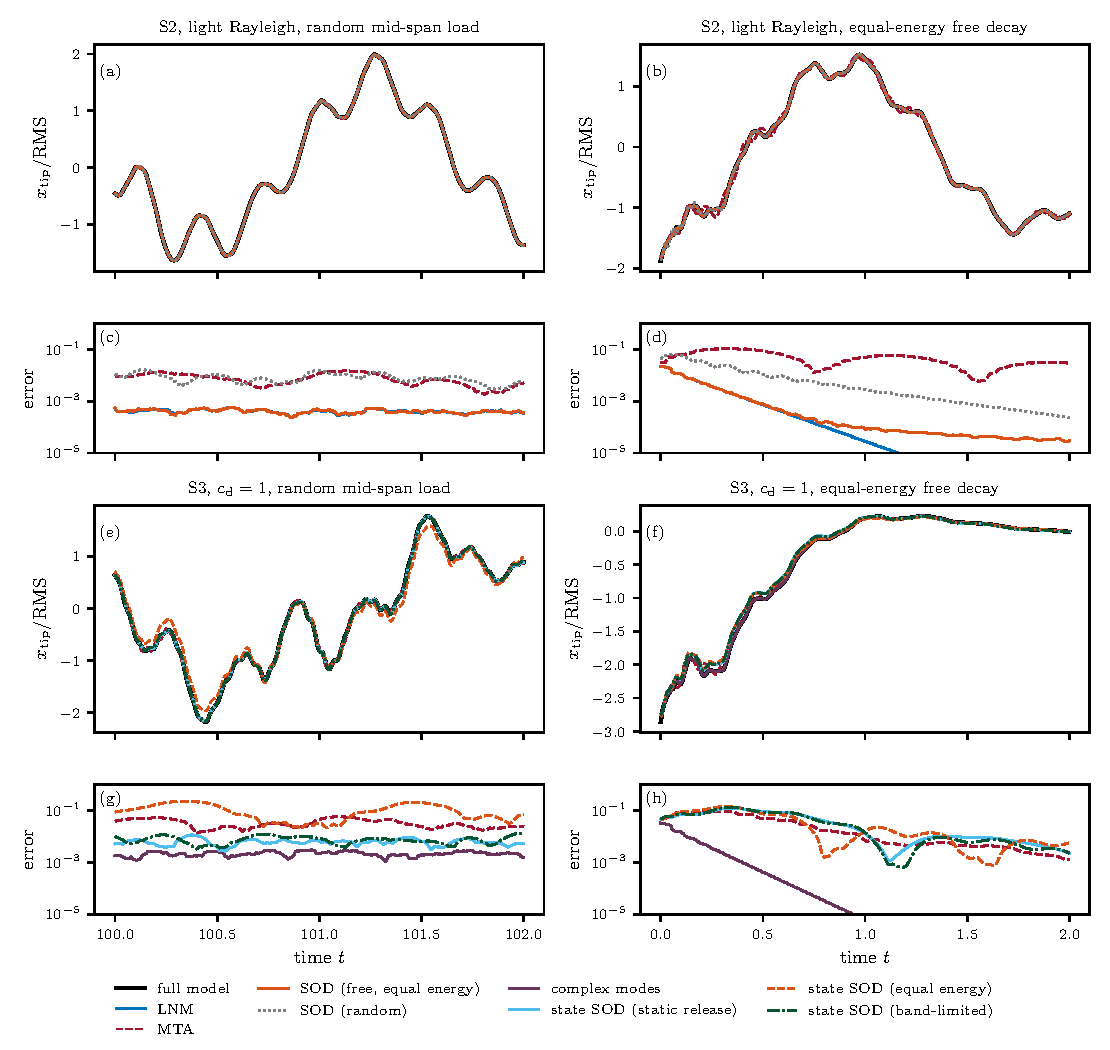
\includegraphics[width=\textwidth]{fig_c_traj.pdf}
\caption{Tip displacement of the full model and ROMs at state dimension 8, one realization. Left: random mid-span load, $t=100$--102. Right: equal-energy test decay ($b_k=(-1)^{k-1}$). (a,b) S2, light Rayleigh damping, configuration ROMs (SOD from the equal-energy decay and from a random tip load). (e,f) S3, $c_{\mathrm d}=1$, state ROMs, MTA and complex modes. (c,d,g,h) Error: root-mean-square (RMS) value of the tip-displacement difference over a sliding 0.1 window. It is divided by the RMS of the full-model tip displacement over the plotted window. Training decays for state SOD: static release, equal energy, and band-limited with $\omega_{\mathrm b}=\omega_4$.}
\label{fig:traj}
\end{figure}

\subsection{Which free decay to train on}\label{sec:ic}
Impact testing aims to excite every mode in the band of interest, with similar force at each frequency. The hammer tip sets that band: a hard tip widens it, a soft tip narrows it. An equal-energy initial state is the numerical analogue of a hard tip. We therefore repeated the free-decay training with EE and BL decays, one realization per case and the ensemble seeds.
Random-trained bases do not depend on the initial state; the random tests reproduce the first ensemble realization.
Away from the data rank, ensemble scatter reached 0.76 of the median. Single-realization differences below a factor of two are therefore not significant.
Figure~\ref{fig:ic} shows the results. For the BL and SR bases, these values agree with the 20-realization medians of Section~\ref{sec:acc} within a factor of 1.25.

\paragraph{Configuration SOD.} Under light Rayleigh damping the initial state hardly mattered on S1 and S2. EE, BL and SR errors agreed within a factor of 1.3 up to $r=5$, and within 2.5 above.
Under heavy Rayleigh damping two effects competed (Figure~\ref{fig:ic}c,d).
\begin{itemize}
\item \emph{Rank.} The static-release decay ended at the data rank: $r=7$ on S1, 6 on S2. EE and BL decays with $\omega_{\mathrm b}=\omega_r$ reached $r=9$ on S2 and the full order on S1.
\item \emph{Accuracy.} At $r=3$--6, EE was 1.3--2.6 times worse than SR on S2 and 2.9--14 times worse on S1. On S1 at $r=4$ it erred by $1.1\times10^{-2}$ against $2.8\times10^{-3}$, and BL with $\omega_{\mathrm b}=\omega_r$ by $5.8\times10^{-3}$.
\end{itemize}
On S3, EE helped configuration SOD at low order. With $c_{\mathrm d}=1$ and the random tip load, it matched complex-mode truncation at $r=2$--4 ($8.1\times10^{-3}$ at $r=4$). The SR basis erred by $2.0\times10^{-2}$.

\paragraph{State-space SOD.} Equal excitation of all modes hurt the state ROMs (Figure~\ref{fig:ic}e,f).
At state dimension 8 and the mid-span load, EE gave $1.3\times10^{-2}$ ($c_{\mathrm d}=0.2$) and $1.2\times10^{-1}$ ($c_{\mathrm d}=1$). SR gave $2.0\times10^{-3}$ and $6.7\times10^{-3}$; complex-mode truncation $1.5\times10^{-3}$ and $3.0\times10^{-3}$.
Band-limiting at $\omega_{\mathrm b}=\omega_r$ restored SR accuracy on forced tests at state dimension 8 and below, within a factor of 1.5. At state dimension 10--16 SR remained best on the random test. At state dimension 12 and $c_{\mathrm d}=1$ it erred by $5.2\times10^{-4}$ on the random test. BL erred by $6.2\times10^{-3}$ and complex modes by $6.7\times10^{-4}$.
Band-limiting at the load cutoff, $\omega_{\mathrm b}=\omega_{\mathrm c}$, still left the state ROMs 2--7 times worse than SR. This held on the forced tests at state dimension 8.

\paragraph{Mechanism.} A transient does not decorrelate the modal planes. Their normalized cross-correlation over a decay from rest depends on damping and frequency spacing, not on record length or amplitude. Its largest value in our records was 0.12 (S2), 0.14 ($c_{\mathrm d}=0.2$) and 0.32--0.34 ($c_{\mathrm d}=1$). It was the same for every initial state that excites modes 1--9.
By Proposition~\ref{prop:ssod}, correlation tilts the smooth planes at first order. The tilt toward a plane outside the ROM grows with that plane's share of the record energy.
We measured the energy-norm leakage of the eight-state SOD subspace out of modal planes 1--4. It was $5.5\times10^{-2}$ (SR), $1.0\times10^{-1}$ (EE) and $2.5\times10^{-1}$ (EE weighted to equal record energy) on S2.
When the leakage exceeded 0.05, the Galerkin ROM converted it into a relative eigenvalue error (Figure~\ref{fig:ic}b). The error was 0.2--0.8 times the leakage squared. At $c_{\mathrm d}=1$, decays with leakage below 0.04 left a floor of $3\times10^{-4}$--$6\times10^{-3}$. With light damping a small frequency error becomes a large response error near resonance. Equal record energy raised the S2 error to $1.7\times10^{-1}$.
The rule for clean data is therefore not equal excitation. It is little energy above the retained band, relative to the energy inside it. Static release meets it because its modal energy falls steeply with mode number (Figure~\ref{fig:ic}a).
Equal excitation helps where rank is scarce: heavy damping, or noise that buries weakly excited modes. Matching the excited band to the ROM order serves both. A hammer tip is matched to the band of interest in the same way.

\paragraph{Free-decay tests of state ROMs.} On the EE test decay, every state SOD ROM erred by $2$--$6\times10^{-2}$ at state dimension 8. This held whether it was trained on the SR, EE or BL decay. Complex modes erred by $5$--$6\times10^{-3}$ (Figure~\ref{fig:traj}h). The cause is the initial state, not the basis. Energy-orthogonal projection maps truncated planes onto retained ones when the modes are complex. Projection with the data covectors was worse, $2.4$--$2.5\times10^{-1}$. Complex-mode truncation uses the exact left eigenvectors.

\begin{figure}[tbp]
\centering
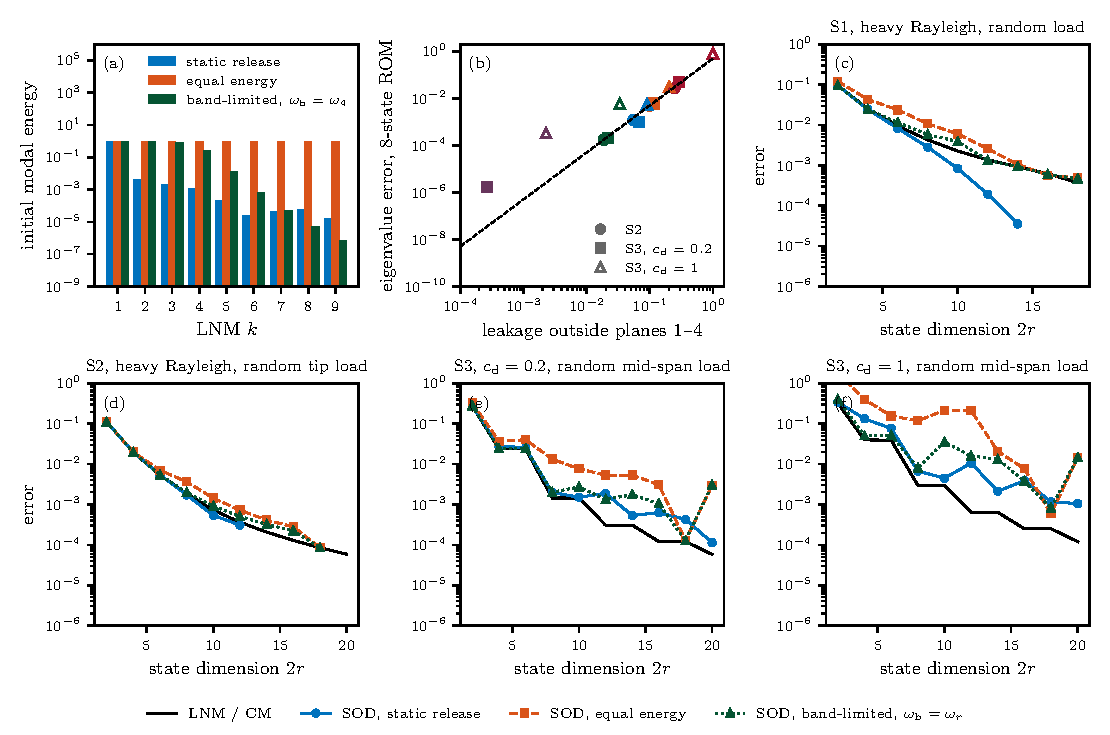
\includegraphics[width=\textwidth]{fig_c_ic.pdf}
\caption{Choice of training decay, one realization. (a) Initial modal energy on the cantilever: static release, equal energy over modes 1--9, and band-limited equal energy with $\omega_{\mathrm b}=\omega_4$. (b) Leakage of the eight-state state-SOD subspace out of modal planes 1--4. It is plotted against the largest relative eigenvalue error of its energy-Galerkin ROM. All training decays are shown (colours as in a; red: equal record energy; plum: modes 1--4 only). Dashed: $0.5\times$ leakage squared. (c,d) Configuration SOD, heavy Rayleigh damping, new random load at the training input. (e,f) State-space SOD on S3, random mid-span load; the solid black line is complex-mode truncation. Band-limited decays use $\omega_{\mathrm b}=\omega_r$.}
\label{fig:ic}
\end{figure}
With complex modes, too, the state-SOD planes follow the record. A decay gives planes tilted toward the modes it excites above the retained band, and a forced record gives planes tilted by its quasi-static response.

\section{The COST F3 cantilever (S4)}\label{sec:s-s4}
\paragraph{Held-out tests over a longer record.} Figure~\ref{fig:nltraj} shows two of these tests over 0.3\,s. At $r=4$ the LNM error grows with time, from phase drift. Over the record it was $1.8\times10^{-2}$ (20\,N tip) and $3.3\times10^{-2}$ (60\,N mid-span). The MTA and SOD errors stay flat, $3.6$--$5.6\times10^{-3}$ over the record, set by the truncated modes.

\begin{figure}[tbp]
\centering
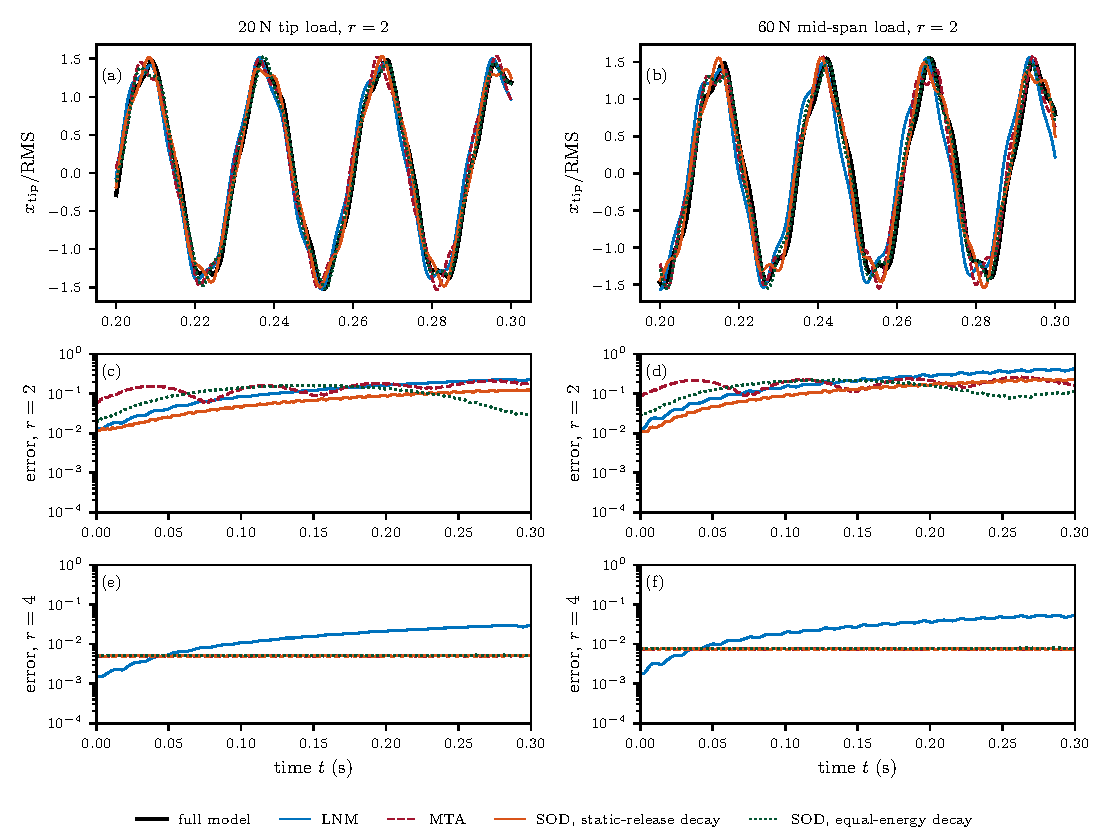
\includegraphics[width=\textwidth]{fig_c_nltraj.pdf}
\caption{COST F3 cantilever, held-out plucked tests released from rest. Static deflection under 20\,N at the tip (left) and 60\,N at mid-span (right). (a,b) Tip displacement of the full model and two-mode ROMs, $t=0.2$--0.3\,s, divided by the RMS full-model tip displacement. (c--f) RMS tip error over a sliding 0.03\,s window (about one period), same normalization: $r=2$ (c,d) and $r=4$ (e,f). SOD bases from the static-release decay (30\,N tip load) and the equal-energy decay (LNMs 1--4).}
\label{fig:nltraj}
\end{figure}
\paragraph{Band-limited training decay.} The band-limited decay starts from an equal-energy sum of LNMs 1--4. Each holds the potential energy of the 30\,N state, $1.48\times10^{-2}$\,J. The total, including the cubic-spring energy, was $8.0\times10^{-2}$\,J.
SOD backbone errors were $5.8\times10^{-3}$, $1.7\times10^{-4}$, $4.9\times10^{-6}$ and $4.1\times10^{-7}$ for $r=1$--4, within a factor of 2.7 of the static-release values. POD was hurt more: $2.8\times10^{-5}$ at $r=4$, against $4\times10^{-7}$.
In the plucked tests the $r=4$ errors were unchanged, $1.6$--$5.5\times10^{-3}$. At $r=2$ they rose to $3.0\times10^{-2}$--$1.1\times10^{-1}$, against $0.8$--$4.8\times10^{-2}$ from static release. As in the linear tests, energy in modes outside a low-order basis costs accuracy.
\paragraph{Tracking the backbone.} Figure~\ref{fig:track}a draws the ROM backbones on the frequency--energy plot. At full scale every two-mode ROM sits on the full-model backbone; all run high as the energy grows. At 0.02\,J the LNM ROM was $5.2\times10^{-3}$ high, MTA and SOD $1.5\times10^{-3}$. At 0.05\,J SOD stayed closest: $3.0\times10^{-3}$, against $6.5\times10^{-3}$ (LNM) and $8.9\times10^{-3}$ (MTA). The four-mode SOD ROM matched to about $10^{-6}$ up to 0.048\,J. There an internal-resonance tongue of the ROM itself begins; the full model's begins at 0.059\,J.
SOD can also read the backbone from the record alone, without a ROM. We slid 0.12\,s windows (3--5 periods) along the static-release decays from 30 and 120\,N. The hop was 0.03\,s.
\begin{itemize}
\item \emph{Configuration SOD:} the frequency of the smoothest coordinate, $\sqrt{\mu_1}/(2\uppi)$.
\item \emph{State SOD:} the NNM1 plane, recognised by circularity, read by the product rule $(\mu_a\mu_b)^{1/4}/(2\uppi)$. NNM1 is taken as the slowest plane whose product-rule frequency agrees with its spectral peak. No reference is used.
\end{itemize}
The state-SOD plane followed the backbone with median errors of $2.6\times10^{-3}$ (30\,N) and $1.2\times10^{-3}$ (120\,N). Its errors were at most $5\times10^{-2}$ (Figure~\ref{fig:track}b,c). Configuration SOD erred by $1.3$--$1.6\times10^{-2}$ in median.
The windows are neither closed nor free of mode 2, which the static release excites strongly. The smoothest configuration coordinate mixes the two. The state plane separates them, because circularity recognises each plane by its own rotation.
\begin{figure}[tbp]
\centering
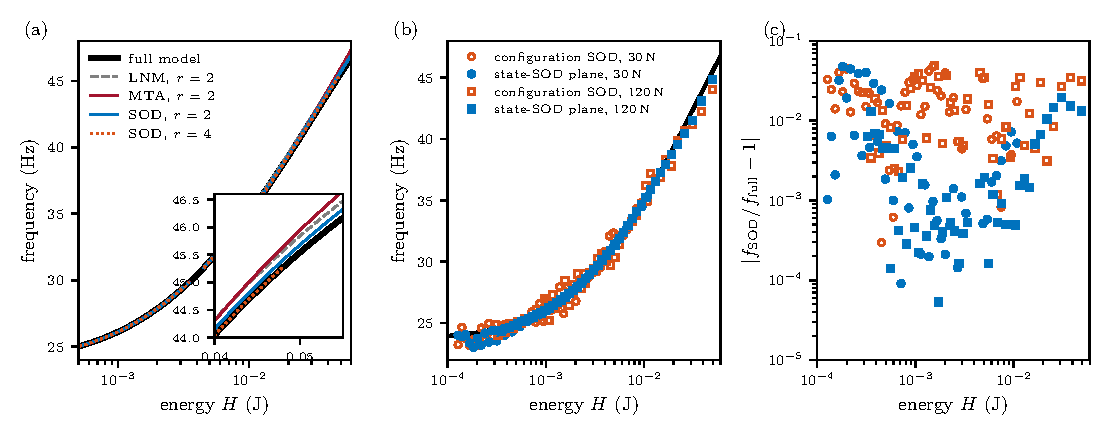
\includegraphics[width=\textwidth]{fig_c_track.pdf}
\caption{COST F3 cantilever (S4): how well SOD follows the NNM1 backbone. (a) Backbones of two-mode ROMs (LNM, MTA, SOD of the 30\,N static-release decay) and of the four-mode SOD ROM. They are drawn on the full-model frequency--energy plot; inset: high-energy end, linear axes. (b) Frequency read from 0.12\,s windows of the decays released from 30\,N (circles) and 120\,N (squares). Open: configuration SOD; filled: the state-SOD NNM1 plane; both against the window energy. (c) Relative frequency error of the window estimates against the full-model backbone.}
\label{fig:track}
\end{figure}
\paragraph{Bending out of the plane.} As the energy rises, the NNM leaves the plane of LNM~1. We applied state SOD to decays released from 30, 60, 120 and 240\,N (initial energies 0.015--0.22\,J). Accelerations came from the equations of motion.
\begin{itemize}
\item Circularity recognised the NNM1 plane in every decay (one-sidedness 0.97--0.99). Spectral consistency on configuration SOD rejected it at 30 and 60\,N. The decay sweeps the NNM frequency, and peak and SOD frequency separated by 10--12\,\%.
\item One non-modal coordinate peaked inside the plane's swept band. Its energy share grew with the load, from $2\times10^{-4}$ to $3.6\times10^{-3}$. With the plane it spans a configuration space $2.1^\circ$ from LNMs 1--2: it is the bend toward mode 2.
\item Band-passed to the swept band, the record had two significant configuration directions, then a drop of 2--3 decades. The state record had four, then a drop by 17--38; the drop after the second value was 4--16. This is consistent with one bend direction, adding one configuration and two state directions. A bent NNM with $\ell$ such directions needs $1+\ell$ configuration and $2+2\ell$ state directions. The bend, and hence $\ell$, depends on amplitude; a decay sweeps through it.
\end{itemize}
At 30\,N the bend also contaminated the mode-2 plane, which then failed the circularity test (0.836). The rule for contaminated planes of Section~\ref{sec:recog} recovered it.
We then ordered a configuration basis by frequency. Each recognised plane enters by its dominant displacement direction, followed by the coordinates peaking in its band. The rest follow in SOD order. Against configuration SOD at $r=2$--4, its backbone error was within 3\,\% or better at every load. At $r=3$ and 60\,N it was $1.8\times10^{-6}$ against $3.9\times10^{-6}$, as low as MTA. On motion started on the NNM it was 2--3 times worse at $r=4$ for 120 and 240\,N.
Frequency and circularity therefore recognise the bent NNM and its out-of-plane direction. As an ordering they helped at 60\,N, by 2.2--3.3 times on the backbone at $r=2$ and 3. Otherwise they changed ROM accuracy little. Configuration SOD's first direction already lies $0.3$--$0.9^\circ$ from $(\bK-\omega^2\bM)^{-1}\bm{e}_{\mathrm{tip}}$, the shape forced at the NNM frequency. Here $\bm{e}_{\mathrm{tip}}$ is the unit load at the tip displacement. The same direction lies $1.1$--$2.7^\circ$ from LNM~1.
\paragraph{Cost.} All models were integrated by average-acceleration Newmark. At $\Delta t=2\times10^{-5}$\,s the full model took 0.89\,s and the LNM, SOD and POD ROMs 0.45--0.58\,s, best of three (\texttt{n2b\_cost\_best3.py}). The differences among ROMs are within the run-to-run spread of up to 27\,\%. Two- and four-mode ROMs took the same time, so per-step overhead, not model size, set it.
The full model and these ROMs held the tip frequency within $10^{-3}$ at $\Delta t=4\times10^{-4}$\,s. The exception was the two-mode POD ROM, which needed $2\times10^{-4}$\,s.
Central differences need $\Delta t<2/\omega_{\max}$: $2.0\times10^{-6}$\,s for the full model and $3.3$--$3.9\times10^{-4}$\,s at $r=4$.
\paragraph{Bent correction vectors on S4.} The first configuration SOD direction of the 30\,N decay lies $2.61^\circ$ from the static tip vector, $1.14^\circ$ from LNM~1 and $3\times10^{-4}$ degrees from $\bm{d}(\omega)=(\bK-\omega^2\bM)^{-1}\bm{e}_{\mathrm{tip}}$ at the first SOD frequency, $\omega=196.0$\,rad/s; the angle is smallest, $9\times10^{-6}$ degrees, at $\omega=196.02$\,rad/s. Table~\ref{tab:s-bent} gives the backbone error of bases built from such vectors. MTA and SOD were recomputed as a control and reproduce the values of Section~\ref{sec:nlbb}. The four-mode SOD subspace and the MTA subspace have principal angles of $1.75^\circ$, $3.4\times10^{-3}$ degrees and less; it holds LNMs 1--3 to relative residuals $9.5\times10^{-6}$, $5.6\times10^{-5}$ and $4.0\times10^{-3}$, and LNM~4 only to 0.35. Sets of four bent vectors at frequencies inside the decay band, and four load-dependent Ritz vectors, were numerically dependent (smallest eigenvalue of the normalized Gram matrix below $10^{-12}$ of the largest), so no basis was formed.

\begin{table}[tbp]
\centering\small
\caption{COST F3 cantilever (S4): median backbone error, outside the 5:1 tongue, of bases built from bent correction vectors $\bm{d}(\omega)$, with $\omega_s=196.0$\,rad/s the first SOD frequency of the 30\,N decay. A dash: the vectors were numerically dependent. Script: \texttt{n14\_bent\_mta.py}.}
\label{tab:s-bent}
\begin{tabular}{lcccc}
\toprule
basis & $r=1$ & 2 & 3 & 4\\ \midrule
MTA: LNMs $1..r-1$, $\bK^{-1}\bm{e}_{\mathrm{tip}}$ & -- & $8.0\times10^{-5}$ & $1.4\times10^{-6}$ & $1.4\times10^{-6}$\\
LNMs $1..r-1$, $\bm{d}(\omega_s)$ & $2.2\times10^{-3}$ & $4.7\times10^{-5}$ & $1.4\times10^{-6}$ & $1.4\times10^{-6}$\\
LNM 1, $\bm{d}(\omega_s)$, $\bm{d}(3\omega_s)$, $\bm{d}(5\omega_s)$ & $1.1\times10^{-2}$ & $4.7\times10^{-5}$ & $1.8\times10^{-6}$ & $1.4\times10^{-6}$\\
LNM 1, $\bm{d}(160)$, $\bm{d}(\omega_s)$, $\bm{d}(228)$ & $1.1\times10^{-2}$ & $6.4\times10^{-5}$ & $2.6\times10^{-6}$ & --\\
load-dependent Ritz vectors \citep{Wilson1982} & $3.6\times10^{-2}$ & $9.4\times10^{-5}$ & $2.7\times10^{-6}$ & --\\
SOD of the 30\,N decay & $2.2\times10^{-3}$ & $1.4\times10^{-4}$ & $2.0\times10^{-6}$ & $5.2\times10^{-7}$\\
\bottomrule
\end{tabular}
\end{table}

\section{The two-well cantilever (S5)}\label{sec:s-s5}
Figure~\ref{fig:mbamp} gives the amplitude diagrams over the whole range swept, and Table~\ref{tab:s-moon} all measures of the amplitude sweep.
\begin{figure}[tbp]
\centering
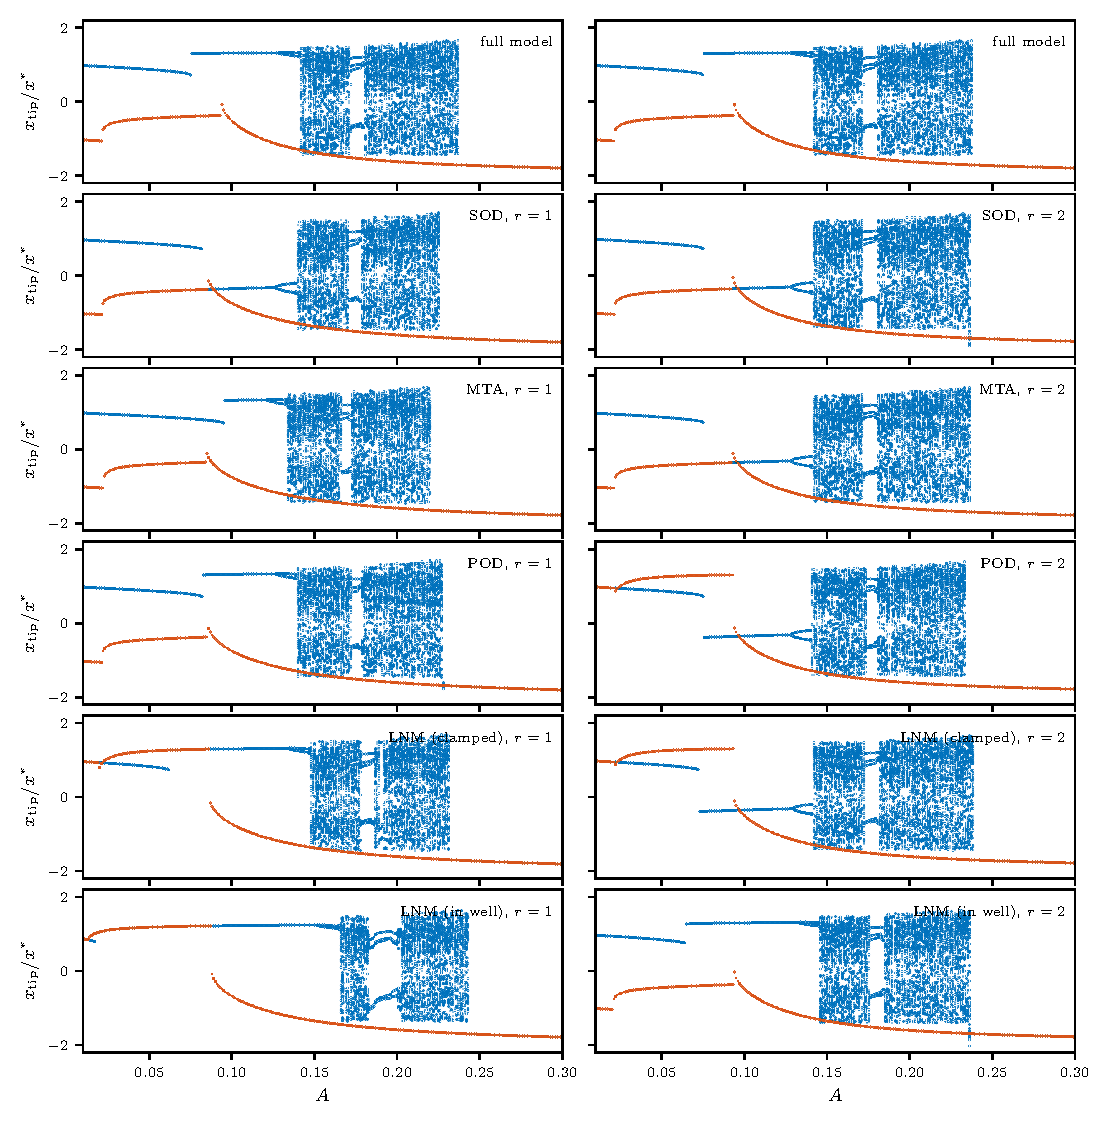
\includegraphics[width=\textwidth]{fig_mb_amp.pdf}
\caption{Two-well beam (S5) at $\varOmega=0.85\,\omega_{\mathrm w}$: amplitude bifurcation diagrams over the whole range swept. Tip displacement sampled once per forcing period, divided by $x^*$; up sweep blue, down sweep orange. Top: full model. Below: ROMs with $r=1$ (left) and $r=2$ (right). Some ROMs settle on the mirror orbit in the other well after the jump near $A=0.075$.}
\label{fig:mbamp}
\end{figure}
\paragraph{Frequency sweep.} At $A=0.3$, $\varOmega$ ran from 0.2 to 1.4 $\omega_{\mathrm w}$ in 121 steps, with 100 transient and 100 sampled periods. The full model was cross-well over most of the range. It was chaotic below $0.45\,\omega_{\mathrm w}$ and, on the down sweep, near $\omega_{\mathrm w}$. Up the sweep it left cross-well motion at $1.325\,\omega_{\mathrm w}$; down the sweep it re-entered at $1.055\,\omega_{\mathrm w}$. At $r\ge2$ every ROM placed these jumps within $0.04\,\omega_{\mathrm w}$. Some ROMs added brief in-well episodes inside the chaotic windows. At one mode all bases but the in-well LNM erred alike. From $r=3$ the ranking of the amplitude sweep returned (Table~\ref{tab:moon}).
\paragraph{The dynamic correction.} The angle between the first SOD direction and $\bm{d}(\omega)=(\bK-\omega^2\bM)^{-1}\bm{e}_{\mathrm{tip}}$, in the mass metric, was $0.69^\circ$ at $\omega=0$, $0.57^\circ$ at 1, $0.22^\circ$ at 2, $0.38^\circ$ at 3, $1.23^\circ$ at 4 and $2.37^\circ$ at 5. Its minimum, $0.003^\circ$, lies at $\omega=2.417$; the first three SOD frequencies were 2.49, 10.4 and 23.8. The basis DMTS replaces the static vector of MTA by $\bm{d}(2.42)$: at $r=1$ it is that vector alone, at $r=2$ the first clamped LNM plus that vector. At $\omega=\omega_{\mathrm w}$ the vector is the in-well LNM, so the one-mode ROM built on it repeats the in-well LNM values of Table~\ref{tab:moon} ($-6.5\,\%$, $-9.3\,\%$).

\begin{table}[tbp]
\centering\small
\caption{Two-well beam, amplitude sweep at $\varOmega=0.85\,\omega_{\mathrm w}$ (step $10^{-3}$, up and down, 582 points). Agreement: share of points whose class (in-well or cross-well, and period up to 16) matches the full model. $W_1$: median Wasserstein distance of the stroboscopic samples, divided by $x^*$, on points in-well in both models and in the same well. Extremes: median error of the in-well orbit extremes, divided by $x^*$ (mirror orbit if the ROM is in the other well). DMTS: MTA with $\bm{d}(2.42)$ in place of the static vector. Scripts: \texttt{mb7\_amp\_compare.py}, \texttt{mb10\_dynamic\_correction.py}.}
\label{tab:s-moon}
\begin{tabular}{llccc}
\toprule
basis & $r$ & agreement (\%) & $W_1$ in-well & extremes\\ \midrule

SOD & 1 & 94.8 & $8.6\times10^{-3}$ & $1.4\times10^{-2}$\\
SOD & 2 & 99.5 & $7.9\times10^{-5}$ & $1.5\times10^{-4}$\\
SOD & 3 & 99.5 & $7.1\times10^{-7}$ & $8.5\times10^{-7}$\\
SOD & 4 & 99.3 & $5.0\times10^{-8}$ & $3.2\times10^{-8}$\\
POD & 1 & 95.7 & $9.0\times10^{-3}$ & $1.4\times10^{-2}$\\
POD & 2 & 98.5 & $6.4\times10^{-4}$ & $1.5\times10^{-4}$\\
POD & 3 & 99.3 & $1.0\times10^{-5}$ & $1.1\times10^{-5}$\\
POD & 4 & 99.3 & $1.9\times10^{-6}$ & $3.8\times10^{-7}$\\
MTA & 1 & 90.4 & $2.5\times10^{-2}$ & $2.6\times10^{-2}$\\
MTA & 2 & 99.5 & $2.0\times10^{-5}$ & $3.2\times10^{-4}$\\
MTA & 3 & 99.5 & $2.3\times10^{-7}$ & $2.4\times10^{-7}$\\
MTA & 4 & 99.5 & $3.2\times10^{-9}$ & $4.8\times10^{-9}$\\
DMTS & 1 & 94.5 & $8.6\times10^{-3}$ & $1.4\times10^{-2}$\\
DMTS & 2 & 99.5 & $1.6\times10^{-5}$ & $3.1\times10^{-4}$\\
LNM, clamped & 1 & 92.8 & $2.0\times10^{-2}$ & $2.0\times10^{-2}$\\
LNM, clamped & 2 & 98.8 & $4.8\times10^{-3}$ & $3.1\times10^{-3}$\\
LNM, clamped & 3 & 99.3 & $8.0\times10^{-4}$ & $9.6\times10^{-4}$\\
LNM, clamped & 4 & 99.5 & $4.1\times10^{-4}$ & $4.1\times10^{-4}$\\
LNM, in well & 1 & 87.5 & $8.8\times10^{-2}$ & $1.2\times10^{-1}$\\
LNM, in well & 2 & 96.9 & $1.2\times10^{-2}$ & $1.5\times10^{-2}$\\
LNM, in well & 3 & 98.5 & $3.6\times10^{-3}$ & $4.5\times10^{-3}$\\
LNM, in well & 4 & 98.6 & $1.7\times10^{-3}$ & $1.9\times10^{-3}$\\
\bottomrule
\end{tabular}
\end{table}

\section{Integration cost at matched integration accuracy}\label{sec:cost}\label{sec:s-cost}
Are SOD ROMs faster, as reported \citep{Ilbeigi2018}, and if so, is the gain a property of SOD?
Two facts frame the answer.
A full-rank change of coordinates is a congruence of $(\bM,\bK)$ and a similarity of the first-order state matrix $\bm{A}$, so it leaves every eigenvalue unchanged.
An explicit integrator is limited by the spectral radius $\rho(\bm{A})$, not only by the highest natural frequency $\omega_{\max}$. With $\bC=\alpha\bM+\beta\bK$ the high finite-element modes are overdamped, and their real eigenvalues, about $\beta\omega^2$, can exceed $\omega_{\max}$. A change of coordinates leaves $\rho(\bm{A})$ unchanged; truncation can lower it.
What a change of coordinates can alter is how an adaptive integrator weighs its error estimate and, for an implicit integrator, how well its Newton iterations are conditioned.
We compared cost at matched integration accuracy. Each model, with each adaptive integrator (RK45 and Radau), was charged its cheapest run whose displacement error against a tight reference of the same model was at most $10^{-6}$ (protocol below; Table~\ref{tab:cost}). This prices integration alone. It does not compare cost against the ROM's total error relative to the full model, which truncation sets; that comparison was not made.

\paragraph{Protocol.} Each model was integrated over 20 (S1) or 10 (S2) periods of mode 1 under a chirp load from $0.5\omega_1$ to $\omega_{\mathrm c}$, with light damping. The SOD and POD bases come from one random record (seed 5).
Every ROM was integrated in Ritz coordinates of its subspace: the eigenvectors of the reduced pencil $(\bm{\varPhi}^{\mathsf T}\bK\bm{\varPhi},\bm{\varPhi}^{\mathsf T}\bM\bm{\varPhi})$, normalized so that the reduced mass is the identity. Under Rayleigh damping the reduced stiffness and damping are then diagonal. The raw smooth modes, with unit Euclidean columns, are kept for one contrast.
Three integrators were used: RK45, the adaptive explicit Runge--Kutta pair of \citet{Dormand1980}; Radau, the implicit fifth-order Radau IIA method \citep{Hairer1996} with analytic Jacobian, both as implemented in SciPy \citep{Virtanen2020}; and central differences at 0.9 of $2/\omega_{\max}$. The central-difference scheme treats damping implicitly, $(\bM/\Delta t^2+\bC/(2\Delta t))\bx_{k+1}=\dots$, so its step limit is $2/\omega_{\max}$ whatever the damping.
Cost is compared at matched integration accuracy. For each model and adaptive integrator, the relative tolerance was swept from $10^{-3}$ to $10^{-9}$ in half decades. Two absolute tolerances were tried at each: one scalar, scaled to the physical response, and one per coordinate, scaled to that coordinate's largest value. The model is charged the run with the fewest function evaluations whose displacement error, against a tight reference of the same model, is at most $10^{-6}$. That run was then timed, best of three, single-threaded. The stiff full cantilever under RK45 is stability-limited at every tolerance and was run once.
All wall times in this paper were measured on one machine: a two-core Intel Xeon at 2.1\,GHz under Linux, with Python 3.13, NumPy 2.5 and SciPy 1.18, on one BLAS thread. The conclusions rest on evaluation and step counts, which do not depend on the machine.

\begin{table}[t]
\centering\small
\caption{Integration cost at matched integration accuracy: the least work to reach a displacement error of $10^{-6}$; light Rayleigh damping, chirp load. ROMs in Ritz coordinates of their subspace; ``raw'' is the same SOD subspace in unit-Euclidean smooth modes. $\rho(\bm{A}_r)$: spectral radius of the first-order state matrix. CD: central-difference steps at 0.9 of $2/\omega_{\max}$. LU: Radau matrix factorizations. --: the single stability-limited RK45 run did not reach $10^{-6}$. Script: \texttt{c36\_cost\_matched.py}, table \texttt{mktab\_c\_cost.py}.}
\label{tab:cost}
\resizebox{\textwidth}{!}{\begin{tabular}{llrrrrrrrr}
\toprule
system & model & $\omega_{\max}$ & $\rho(\bm{A}_r)$ & CD steps & RK45 evals & RK45 (s) & Radau evals & Radau LU & Radau (s)\\
\midrule
S1 & full, physical & 36.2 & 36.2 & 924 & 13\,562 & 0.23 & 13\,342 & 244 & 0.47\\
 & full, LNM coordinates & 36.2 & 36.2 & 924 & 12\,020 & 0.15 & 14\,729 & 212 & 0.39\\
 & LNM $r=4$ & 17.1 & 17.1 & 436 & 10\,922 & 0.14 & 15\,406 & 36 & 0.40\\
 & MTA $r=4$ & 18.9 & 18.9 & 483 & 12\,056 & 0.20 & 12\,967 & 448 & 0.40\\
 & POD $r=4$ & 17.1 & 17.1 & 436 & 10\,970 & 0.14 & 15\,559 & 40 & 0.47\\
 & SOD $r=4$ & 17.7 & 17.7 & 453 & 11\,540 & 0.15 & 15\,497 & 36 & 0.49\\
 & LNM $r=8$ & 30.6 & 30.6 & 780 & 12\,770 & 0.17 & 15\,236 & 222 & 0.45\\
 & MTA $r=8$ & 32.5 & 32.5 & 828 & 11\,168 & 0.19 & 14\,204 & 96 & 0.50\\
 & POD $r=8$ & 32.4 & 32.4 & 827 & 11\,168 & 0.14 & 14\,140 & 84 & 0.49\\
 & SOD $r=8$ & 32.9 & 32.9 & 838 & 11\,150 & 0.19 & 15\,169 & 228 & 0.44\\
 & SOD $r=8$, raw smooth modes & 32.9 & 32.9 & 838 & 13\,592 & 0.23 & 14\,353 & 124 & 0.37\\
\midrule
S2 & full, physical & $5.4\times10^{4}$ & $9.3\times10^{5}$ & 535\,013 & 35\,062\,052 & 471.22 & 62\,792 & 1\,760 & 3.19\\
 & full, LNM coordinates & $5.4\times10^{4}$ & $9.3\times10^{5}$ & 535\,013 & -- & -- & 58\,946 & 3\,350 & 4.00\\
 & LNM $r=4$ & 121 & 121 & 1\,201 & 40\,214 & 0.58 & 55\,920 & 3\,842 & 1.89\\
 & MTA $r=4$ & 135 & 135 & 1\,338 & 36\,002 & 0.40 & 62\,596 & 2\,922 & 1.99\\
 & POD $r=4$ & 121 & 121 & 1\,204 & 40\,790 & 0.61 & 56\,426 & 3\,920 & 1.92\\
 & SOD $r=4$ & 169 & 169 & 1\,679 & 44\,990 & 0.51 & 57\,876 & 52 & 1.74\\
 & LNM $r=8$ & 555 & 555 & 5\,514 & 53\,636 & 0.67 & 57\,290 & 3\,394 & 1.70\\
 & MTA $r=8$ & 717 & 717 & 7\,124 & 59\,834 & 0.85 & 57\,093 & 3\,316 & 2.02\\
 & POD $r=8$ & 882 & 882 & 8\,755 & 72\,416 & 0.77 & 57\,182 & 3\,346 & 1.68\\
 & SOD $r=8$ & 882 & 882 & 8\,755 & 72\,386 & 0.90 & 57\,151 & 3\,344 & 1.50\\
 & SOD $r=8$, raw smooth modes & 882 & 882 & 8\,755 & 71\,378 & 0.86 & 110\,084 & 6\,792 & 3.20\\
\bottomrule
\end{tabular}
% times: two-core Linux workspace, 14 Nov 2026
}
\end{table}

\begin{itemize}
\item \emph{Truncation sets the cost.} On S2 the full model is limited by its largest eigenvalue, real and equal to $-9.3\times10^5$: an overdamped finite-element mode under the $\beta\bK$ term, 17 times $\omega_{\max}$. RK45 needed $3.5\times10^7$ evaluations to reach $10^{-6}$; the four-mode LNM ROM needed $4.0\times10^4$, about 870 times fewer. Central-difference steps fell from 535\,013 to 1\,201. Radau is not stability-limited: it needed $6.3\times10^4$ evaluations for the full model and $5.6$--$6.3\times10^4$ for every ROM in Ritz coordinates.
\item \emph{Coordinates do not, at matched integration accuracy.} The order-8 SOD subspace of S2 needed 72\,386 RK45 evaluations in Ritz coordinates and 71\,378 in raw smooth modes; on S1 the raw basis needed 1.2 times as many. For Radau the raw smooth modes needed 1.9 times the evaluations and 2.0 times the factorizations of Ritz coordinates on S2. Their reduced mass matrix has condition number $7.4\times10^6$; in Ritz coordinates it is the identity. The full model needed 58\,946 Radau evaluations in LNM coordinates and 62\,792 in physical ones.
\item \emph{A fixed tolerance misleads.} At one fixed setting (relative tolerance $10^{-6}$, absolute $10^{-9}$), the order-8 SOD subspace of S2 needed 416\,k RK45 evaluations in raw smooth modes and 158\,k in Ritz coordinates, but the two runs reached errors of $2.1\times10^{-10}$ and $3.8\times10^{-9}$. At that setting Radau took 11.3\,s for the full model and 3.8\,s in LNM coordinates, at errors of $1.5\times10^{-8}$ and $4.8\times10^{-8}$ (\texttt{k1\_basis\_cost.py}, \texttt{k2\_matched\_cost.py}). An absolute tolerance weighs coordinates by their scale, and a change of coordinates changes the scale.
\item \emph{The SOD subspace is slightly stiffer.} The quasi-static direction raises the projected $\omega_{\max}$: 169 against 121 at $r=4$, and 882 against 555 at $r=8$, where SOD and POD span one subspace. At $10^{-6}$ the order-8 SOD ROM needed 1.35 times the RK45 evaluations of the LNM ROM. At $10^{-8}$, where accuracy limits the step, it needed 0.94 times as many (131\,684 against 139\,832). Radau cost the same for both.
\item \emph{Load bandwidth.} On S1 the chirp reaches $\omega_{\mathrm c}=23$, close to $\omega_{\max}=36.2$. Accuracy, not stability, then limits the step, and every model, the full one included, cost the same within 25\,\% (Table~\ref{tab:cost}).
\end{itemize}
\citet{Ilbeigi2018} studied a ten-dimensional, full-order SOD model of a nonlinear control system and reported that it ran about twice as fast as the original. A full-rank linear change of coordinates cannot change the eigenvalues. At a fixed tolerance, the coordinate scaling alone produced differences of that size here, and at matched integration accuracy they vanished. We have not tested their system.
For SOD ROMs we recommend Ritz coordinates of the retained subspace: they decouple the reduced model and, in every case tested, were no costlier than any other basis of the same subspace.

\bibliographystyle{elsarticle-num-names}
\bibliography{../refs}
\end{document}
